\chapter{Operations on Images}

\section{Pixel Connectivity}
The relationship between two or more pixels is defined as Pixel Connectivity.
Connectivity information is used to establish the boundaries of the objects.
The pixels $p$ and $q$ are said to be connected if certain conditions on pixel brightness specified by the set $V$ and spatial adjacency are satisfied.
For a binary image, this set $V$ will be $\{0,1\}$ and for grayscale images, $V$ might be of any range of Gray Levels.

\subsubsection{4-Connectivity:}
The pixels $p$ and $q$ are said to be in 4-connectivity when both have the same values as specified by the set $V$ and if $q$ is said to be in the set $N_4(p)$. This implies any path from $p$ to $q$ on which every other pixel is 4-connected to the next pixel.

In terms of pixel coordinates,
$$(x \pm 1, y) or (x, y \pm 1)$$

\subsubsection{6-Connectivity:}

6-connected pixels are neighbours to every pixel that touches one of their corners in a hexagonal grid or stretcher bond rectangular grid.
There are several ways to map hexagonal tiles to integer pixel coordinates.
With one method, in addition to the 4-connected pixels, the two additional pixel coordinates $$(x+1, y+1) and (x-1, y-1)$$ are connected to the pixel at $(x,y)$.

\subsubsection{8-Connectivity:}
It is assumed that the pixels $p$ and $q$ share a common grayscale value. The pixels $p$ and $q$ are said to be in 8-connectivity if $q$ is in the set $N_8(p)$.
In simpler terms, in addition to 4-connected pixels, each pixel with coordinates $$(x \pm 1, y \pm 1)$$ is connected to the pixel at $(x,y)$.
Eg: Fig: \ref{8-connectivity} shows 8-connectivity when $V = \{0,1\}$. Here, a multiple path or Loop is present.

\begin{figure}[h]
    \centering
    \tikzset{every picture/.style={line width=0.75pt}} %set default line width to 0.75pt        

    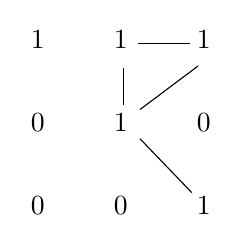
\begin{tikzpicture}[x=0.75pt,y=0.75pt,yscale=-1,xscale=1]
    %uncomment if require: \path (0,300); %set diagram left start at 0, and has height of 300

    %Straight Lines [id:da23478130696835353] 
    \draw    (77.8,45.2) -- (77.8,63.2) ;
    %Straight Lines [id:da8259417229972419] 
    \draw    (84.8,33.2) -- (109.8,33.2) ;
    %Straight Lines [id:da8853039395054243] 
    \draw    (85.8,65.2) -- (113.8,44.2) ;
    %Straight Lines [id:da02549560843434784] 
    \draw    (85.8,79.2) -- (110.8,105.2) ;

    % Text Node
    \draw (32,26) node [anchor=north west][inner sep=0.75pt]   [align=left] {1};
    % Text Node
    \draw (32,66) node [anchor=north west][inner sep=0.75pt]   [align=left] {0};
    % Text Node
    \draw (32,106) node [anchor=north west][inner sep=0.75pt]   [align=left] {0};
    % Text Node
    \draw (72,26) node [anchor=north west][inner sep=0.75pt]   [align=left] {1};
    % Text Node
    \draw (72,66) node [anchor=north west][inner sep=0.75pt]   [align=left] {1};
    % Text Node
    \draw (72,106) node [anchor=north west][inner sep=0.75pt]   [align=left] {0};
    % Text Node
    \draw (112,26) node [anchor=north west][inner sep=0.75pt]   [align=left] {1};
    % Text Node
    \draw (112,66) node [anchor=north west][inner sep=0.75pt]   [align=left] {0};
    % Text Node
    \draw (112,106) node [anchor=north west][inner sep=0.75pt]   [align=left] {1};

    \end{tikzpicture}

    \caption{8-Connectivity represented as lines}
    \label{8-connectivity}
\end{figure}

\subsubsection{Mixed Connectivity:}
Mixed Connectivity is also known as $m$-connectivity.
Two pixels $p$ and $q$ are said to be in $m$-connectivity when ---
\begin{enumerate}
    \item $q$ is in $N_4(p)$ or
    \item $q$ is in $N_D(p)$ and the intesection of $N_4(p)$ and $N_4(q)$ is empty.
\end{enumerate}

Eg: Fig: \ref{m-connectivity} shows an $m$-connectivity that there is no multiple paths or loops present in the connectivity. It can be observed that multiple paths have been removed.

\begin{figure}[h]
    \centering

    \tikzset{every picture/.style={line width=0.75pt}} %set default line width to 0.75pt        

    \begin{tikzpicture}[x=0.75pt,y=0.75pt,yscale=-1,xscale=1]
    %uncomment if require: \path (0,165); %set diagram left start at 0, and has height of 165
    
    %Straight Lines [id:da38565778933018646] 
    \draw    (207.8,45.2) -- (207.8,63.2) ;
    %Straight Lines [id:da331753409787636] 
    \draw    (214.8,33.2) -- (239.8,33.2) ;
    %Straight Lines [id:da5176626800362345] 
    \draw    (215.8,79.2) -- (240.8,105.2) ;
    
    % Text Node
    \draw (162,26) node [anchor=north west][inner sep=0.75pt]   [align=left] {1};
    % Text Node
    \draw (162,66) node [anchor=north west][inner sep=0.75pt]   [align=left] {0};
    % Text Node
    \draw (162,106) node [anchor=north west][inner sep=0.75pt]   [align=left] {0};
    % Text Node
    \draw (202,26) node [anchor=north west][inner sep=0.75pt]   [align=left] {1};
    % Text Node
    \draw (202,66) node [anchor=north west][inner sep=0.75pt]   [align=left] {1};
    % Text Node
    \draw (202,106) node [anchor=north west][inner sep=0.75pt]   [align=left] {0};
    % Text Node
    \draw (242,26) node [anchor=north west][inner sep=0.75pt]   [align=left] {1};
    % Text Node
    \draw (242,66) node [anchor=north west][inner sep=0.75pt]   [align=left] {0};
    % Text Node
    \draw (242,106) node [anchor=north west][inner sep=0.75pt]   [align=left] {1};
    
    \end{tikzpicture}

    \caption{$m$-connectivity}
    \label{m-connectivity}
\end{figure}

\section{Distance Measures}

The distance between the pixels $p$ and $q$ in an image can be given by distance measures such as Euclidean Distance, $D_4$ distance and $D_8$ distance.

Consider three pixels $p$,$q$ and $z$.
If the coordinates of the pixels are $P(x,y)$, $Q(s,t)$ and $Z(u,w)$ as shown in Fig: \ref{distanceSample}, the distances between the pixels can be calculated.

\begin{figure}[h]
    \centering

    \begin{equation*}
        \begin{matrix}
        0 & 1 & 1 & 1 & ( z)\\
        1 & 0 & 0 & 1 & \\
        1 & 1 & 1 & 1 & ( q)\\
        1 & 1 & 1 & 1 & \\
        ( p) &  &  &  & 
        \end{matrix}
    \end{equation*}

    \caption{Sample Image}
    \label{distanceSample}
\end{figure}

The distance function can be called \textit{Metric}, if the following properties are satisfied:
\begin{enumerate}
    \item $D(p,q)$ is well-defined and finite for all $p$ and $q$.
    \item $D(p,q) \geqslant 0$ if $p = q$, then $D(p,q)=0$.
    \item The distance $D(p,q) = D(q,p)$.
    \item $D(p,q) + D(q,z) \geqslant D(p,z)$. This is called property of triangular inequality.
\end{enumerate}

\subsubsection{Euclidean Distance:}
The Euclidean Distance between the pixels $p$ and $q$, with coordinates $(x,y)$ and $(s,t)$, respectively, can be defined as:
$$D_e(p,q) = \sqrt{(x-s)^2+(y-t)^2}$$
The advantage of Euclidean Distance is its simplicity.
However it is very computationally costly due to involvement of square root operations.

\subsubsection{$D_4$ Distance or City Block Distance:}
The $D_4$ distance or City Block Distance can be simply calculated as:
$$D_4(p,q) = |x-s| + |y-t|$$

\subsubsection{$D_8$ Distance or Chessboard Distance:}
This is calculated with the help of the following:
$$D_8(p,q) = \max (|x-s|, |y-t|)$$

\subsubsection{Question:}
Let $V = \{0,1\}$. Compute the $D_e$, $D_4$, $D_8$ and $D_m$ distances between two pixels $p$ and $q$. Let the pixel coordinates of $p$ and $q$ be $(3,0)$ and $(2,3)$ respectively, for the image shown below. Find the Distance Measures.

\begin{figure}[h]
    \centering

    \tikzset{every picture/.style={line width=0.75pt}} %set default line width to 0.75pt        

    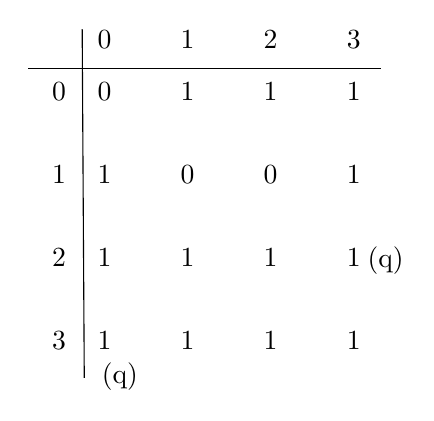
\begin{tikzpicture}[x=0.75pt,y=0.75pt,yscale=-1,xscale=1]
    %uncomment if require: \path (0,231); %set diagram left start at 0, and has height of 231
    
    %Straight Lines [id:da031132642263489663] 
    \draw    (19.8,40.4) -- (189.8,40.4) ;
    %Straight Lines [id:da9944079929840195] 
    \draw    (45.8,21.4) -- (46.8,189.4) ;
    
    % Text Node
    \draw (52,46) node [anchor=north west][inner sep=0.75pt]   [align=left] {0};
    % Text Node
    \draw (52,86) node [anchor=north west][inner sep=0.75pt]   [align=left] {1};
    % Text Node
    \draw (52,126) node [anchor=north west][inner sep=0.75pt]   [align=left] {1};
    % Text Node
    \draw (92,46) node [anchor=north west][inner sep=0.75pt]   [align=left] {1};
    % Text Node
    \draw (92,86) node [anchor=north west][inner sep=0.75pt]   [align=left] {0};
    % Text Node
    \draw (92,126) node [anchor=north west][inner sep=0.75pt]   [align=left] {1};
    % Text Node
    \draw (132,46) node [anchor=north west][inner sep=0.75pt]   [align=left] {1};
    % Text Node
    \draw (132,86) node [anchor=north west][inner sep=0.75pt]   [align=left] {0};
    % Text Node
    \draw (132,126) node [anchor=north west][inner sep=0.75pt]   [align=left] {1};
    % Text Node
    \draw (172,46) node [anchor=north west][inner sep=0.75pt]   [align=left] {1};
    % Text Node
    \draw (172,86) node [anchor=north west][inner sep=0.75pt]   [align=left] {1};
    % Text Node
    \draw (172,126) node [anchor=north west][inner sep=0.75pt]   [align=left] {1};
    % Text Node
    \draw (52,166) node [anchor=north west][inner sep=0.75pt]   [align=left] {1};
    % Text Node
    \draw (92,166) node [anchor=north west][inner sep=0.75pt]   [align=left] {1};
    % Text Node
    \draw (132,166) node [anchor=north west][inner sep=0.75pt]   [align=left] {1};
    % Text Node
    \draw (172,166) node [anchor=north west][inner sep=0.75pt]   [align=left] {1};
    % Text Node
    \draw (182,125) node [anchor=north west][inner sep=0.75pt]   [align=left] {(q)};
    % Text Node
    \draw (54,181) node [anchor=north west][inner sep=0.75pt]   [align=left] {(q)};
    % Text Node
    \draw (52,21) node [anchor=north west][inner sep=0.75pt]   [align=left] {0};
    % Text Node
    \draw (92,21) node [anchor=north west][inner sep=0.75pt]   [align=left] {1};
    % Text Node
    \draw (132,21) node [anchor=north west][inner sep=0.75pt]   [align=left] {2};
    % Text Node
    \draw (172,21) node [anchor=north west][inner sep=0.75pt]   [align=left] {3};
    % Text Node
    \draw (30,46) node [anchor=north west][inner sep=0.75pt]   [align=left] {0};
    % Text Node
    \draw (30,86) node [anchor=north west][inner sep=0.75pt]   [align=left] {1};
    % Text Node
    \draw (30,126) node [anchor=north west][inner sep=0.75pt]   [align=left] {2};
    % Text Node
    \draw (30,166) node [anchor=north west][inner sep=0.75pt]   [align=left] {3};
    
    \end{tikzpicture}

    \caption{Sample Image}
    \label{question3_1}
\end{figure}

\textbf{Solution:}\\

The Euclidean Distance is:

\begin{equation*}
    \begin{aligned}
    D_e & = \sqrt{( x-s)^{2} +( y-t)^{2}}\\
        & = \sqrt{( 3-2)^{2} +( 0-3)^{2}}\\
        & = \sqrt{1+9}\\
        & = \sqrt{10}
    \end{aligned}
\end{equation*}

\begin{equation*}
    \begin{aligned}
    D_4 & = \sqrt{|x-s| + |y-t|}\\
        & = |3-2| + |0-3|\\
        & = 1 + 3\\
        & = 4
    \end{aligned}
\end{equation*}

\begin{equation*}
    \begin{aligned}
    D_8 & = max(|x-s|, |y-t|)\\
        & = max(|3-2|, |0-3|)\\
        & = max(1,3)
    \end{aligned}
\end{equation*}

The distances can be checked with Fig: \ref{question3_abcd}.

The distance $D_m$ depends on the values of the set $V$. The implications of the set $V$ is that the path should be constructed only using the elements of $V$. So if the value of the set are changed, the path also changes.

The simplest $D_m$ distance can be calculated along the diagonal path. Here the distance is 3. Suppose the set $V = \{1\}$, the path of the distance $D_m$ also changes.

\begin{figure}[h]
    \centering


    \tikzset{every picture/.style={line width=0.75pt}} %set default line width to 0.75pt        

    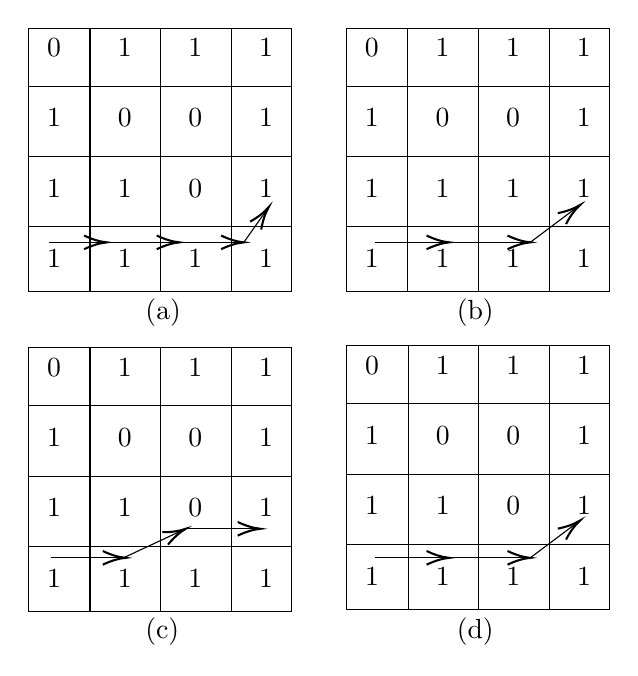
\begin{tikzpicture}[x=0.75pt,y=0.75pt,yscale=-1,xscale=1]
    %uncomment if require: \path (0,518); %set diagram left start at 0, and has height of 518
    
    %Shape: Rectangle [id:dp4475078963739587] 
    \draw   (40.97,18) -- (167.55,18) -- (167.55,145.03) -- (40.97,145.03) -- cycle ;
    %Straight Lines [id:da2837534659997365] 
    \draw    (70.57,18) -- (70.57,145.03) ;
    %Straight Lines [id:da08026350336095867] 
    \draw    (104.6,18) -- (104.6,145.03) ;
    %Straight Lines [id:da12341745735028331] 
    \draw    (138.63,18) -- (138.63,145.03) ;
    %Straight Lines [id:da18544345546390129] 
    \draw    (40.8,45.95) -- (167.55,45.95) ;
    %Straight Lines [id:da36332599792717035] 
    \draw    (40.8,79.82) -- (167.55,79.82) ;
    %Straight Lines [id:da24591625396036432] 
    \draw    (40.8,113.7) -- (167.55,113.7) ;
    %Shape: Rectangle [id:dp662906702606036] 
    \draw   (194.09,18) -- (320.68,18) -- (320.68,145.03) -- (194.09,145.03) -- cycle ;
    %Straight Lines [id:da12263567220380134] 
    \draw    (223.7,18) -- (223.7,145.03) ;
    %Straight Lines [id:da9762779391264798] 
    \draw    (257.73,18) -- (257.73,145.03) ;
    %Straight Lines [id:da8391602158100666] 
    \draw    (291.75,18) -- (291.75,145.03) ;
    %Straight Lines [id:da3444859343840154] 
    \draw    (193.92,45.95) -- (320.68,45.95) ;
    %Straight Lines [id:da09476418356870342] 
    \draw    (193.92,79.82) -- (320.68,79.82) ;
    %Straight Lines [id:da3655568500531654] 
    \draw    (193.92,113.7) -- (320.68,113.7) ;
    %Shape: Rectangle [id:dp8791357369590893] 
    \draw   (194.22,171) -- (320.8,171) -- (320.8,298.03) -- (194.22,298.03) -- cycle ;
    %Straight Lines [id:da05710193912163852] 
    \draw    (223.82,171) -- (223.82,298.03) ;
    %Straight Lines [id:da5717774023965383] 
    \draw    (257.85,171) -- (257.85,298.03) ;
    %Straight Lines [id:da25157700320628273] 
    \draw    (291.88,171) -- (291.88,298.03) ;
    %Straight Lines [id:da2995322489461316] 
    \draw    (194.05,198.95) -- (320.8,198.95) ;
    %Straight Lines [id:da6641804756632277] 
    \draw    (194.05,232.82) -- (320.8,232.82) ;
    %Straight Lines [id:da41797334591979096] 
    \draw    (194.05,266.7) -- (320.8,266.7) ;
    %Shape: Rectangle [id:dp4396916259579262] 
    \draw   (40.97,171.97) -- (167.55,171.97) -- (167.55,299) -- (40.97,299) -- cycle ;
    %Straight Lines [id:da052648741807676425] 
    \draw    (70.57,171.97) -- (70.57,299) ;
    %Straight Lines [id:da064462116667372] 
    \draw    (104.6,171.97) -- (104.6,299) ;
    %Straight Lines [id:da9610667135321806] 
    \draw    (138.63,171.97) -- (138.63,299) ;
    %Straight Lines [id:da384489478960784] 
    \draw    (40.8,199.92) -- (167.55,199.92) ;
    %Straight Lines [id:da9740468772342308] 
    \draw    (40.8,233.79) -- (167.55,233.79) ;
    %Straight Lines [id:da9410970713310336] 
    \draw    (40.8,267.67) -- (167.55,267.67) ;
    %Straight Lines [id:da4991960651404055] 
    \draw    (50.67,121.17) -- (76.67,121.17) ;
    \draw [shift={(78.67,121.17)}, rotate = 180] [color={rgb, 255:red, 0; green, 0; blue, 0 }  ][line width=0.75]    (10.93,-3.29) .. controls (6.95,-1.4) and (3.31,-0.3) .. (0,0) .. controls (3.31,0.3) and (6.95,1.4) .. (10.93,3.29)   ;
    %Straight Lines [id:da40533492288555495] 
    \draw    (77.67,121.17) -- (111.67,121.17) ;
    \draw [shift={(113.67,121.17)}, rotate = 180] [color={rgb, 255:red, 0; green, 0; blue, 0 }  ][line width=0.75]    (10.93,-3.29) .. controls (6.95,-1.4) and (3.31,-0.3) .. (0,0) .. controls (3.31,0.3) and (6.95,1.4) .. (10.93,3.29)   ;
    %Straight Lines [id:da5889055549592568] 
    \draw    (113.67,121.17) -- (142.67,121.17) ;
    \draw [shift={(144.67,121.17)}, rotate = 180] [color={rgb, 255:red, 0; green, 0; blue, 0 }  ][line width=0.75]    (10.93,-3.29) .. controls (6.95,-1.4) and (3.31,-0.3) .. (0,0) .. controls (3.31,0.3) and (6.95,1.4) .. (10.93,3.29)   ;
    %Straight Lines [id:da9582772307945706] 
    \draw    (144.67,121.17) -- (155.51,105.8) ;
    \draw [shift={(156.67,104.17)}, rotate = 485.22] [color={rgb, 255:red, 0; green, 0; blue, 0 }  ][line width=0.75]    (10.93,-3.29) .. controls (6.95,-1.4) and (3.31,-0.3) .. (0,0) .. controls (3.31,0.3) and (6.95,1.4) .. (10.93,3.29)   ;
    %Straight Lines [id:da23239242378169922] 
    \draw    (207.67,121.17) -- (241.67,121.17) ;
    \draw [shift={(243.67,121.17)}, rotate = 180] [color={rgb, 255:red, 0; green, 0; blue, 0 }  ][line width=0.75]    (10.93,-3.29) .. controls (6.95,-1.4) and (3.31,-0.3) .. (0,0) .. controls (3.31,0.3) and (6.95,1.4) .. (10.93,3.29)   ;
    %Straight Lines [id:da30210328263691966] 
    \draw    (243.67,121.17) -- (280.67,121.17) ;
    \draw [shift={(282.67,121.17)}, rotate = 180] [color={rgb, 255:red, 0; green, 0; blue, 0 }  ][line width=0.75]    (10.93,-3.29) .. controls (6.95,-1.4) and (3.31,-0.3) .. (0,0) .. controls (3.31,0.3) and (6.95,1.4) .. (10.93,3.29)   ;
    %Straight Lines [id:da27150216124144677] 
    \draw    (282.67,121.17) -- (305.07,104.37) ;
    \draw [shift={(306.67,103.17)}, rotate = 503.13] [color={rgb, 255:red, 0; green, 0; blue, 0 }  ][line width=0.75]    (10.93,-3.29) .. controls (6.95,-1.4) and (3.31,-0.3) .. (0,0) .. controls (3.31,0.3) and (6.95,1.4) .. (10.93,3.29)   ;
    %Straight Lines [id:da5600081587944892] 
    \draw    (207.67,273.17) -- (241.67,273.17) ;
    \draw [shift={(243.67,273.17)}, rotate = 180] [color={rgb, 255:red, 0; green, 0; blue, 0 }  ][line width=0.75]    (10.93,-3.29) .. controls (6.95,-1.4) and (3.31,-0.3) .. (0,0) .. controls (3.31,0.3) and (6.95,1.4) .. (10.93,3.29)   ;
    %Straight Lines [id:da07105978503613741] 
    \draw    (243.67,273.17) -- (280.67,273.17) ;
    \draw [shift={(282.67,273.17)}, rotate = 180] [color={rgb, 255:red, 0; green, 0; blue, 0 }  ][line width=0.75]    (10.93,-3.29) .. controls (6.95,-1.4) and (3.31,-0.3) .. (0,0) .. controls (3.31,0.3) and (6.95,1.4) .. (10.93,3.29)   ;
    %Straight Lines [id:da8864300844744744] 
    \draw    (282.67,273.17) -- (305.07,256.37) ;
    \draw [shift={(306.67,255.17)}, rotate = 503.13] [color={rgb, 255:red, 0; green, 0; blue, 0 }  ][line width=0.75]    (10.93,-3.29) .. controls (6.95,-1.4) and (3.31,-0.3) .. (0,0) .. controls (3.31,0.3) and (6.95,1.4) .. (10.93,3.29)   ;
    %Straight Lines [id:da03005048226319551] 
    \draw    (51.67,273.17) -- (85.67,273.17) ;
    \draw [shift={(87.67,273.17)}, rotate = 180] [color={rgb, 255:red, 0; green, 0; blue, 0 }  ][line width=0.75]    (10.93,-3.29) .. controls (6.95,-1.4) and (3.31,-0.3) .. (0,0) .. controls (3.31,0.3) and (6.95,1.4) .. (10.93,3.29)   ;
    %Straight Lines [id:da06389652649955102] 
    \draw    (116.67,259.17) -- (150.67,259.17) ;
    \draw [shift={(152.67,259.17)}, rotate = 180] [color={rgb, 255:red, 0; green, 0; blue, 0 }  ][line width=0.75]    (10.93,-3.29) .. controls (6.95,-1.4) and (3.31,-0.3) .. (0,0) .. controls (3.31,0.3) and (6.95,1.4) .. (10.93,3.29)   ;
    %Straight Lines [id:da3962475595082513] 
    \draw    (86.67,273.17) -- (114.85,260.01) ;
    \draw [shift={(116.67,259.17)}, rotate = 514.98] [color={rgb, 255:red, 0; green, 0; blue, 0 }  ][line width=0.75]    (10.93,-3.29) .. controls (6.95,-1.4) and (3.31,-0.3) .. (0,0) .. controls (3.31,0.3) and (6.95,1.4) .. (10.93,3.29)   ;
    
    % Text Node
    \draw (48.66,21.78) node [anchor=north west][inner sep=0.75pt]   [align=left] {0};
    % Text Node
    \draw (48.66,55.65) node [anchor=north west][inner sep=0.75pt]   [align=left] {1};
    % Text Node
    \draw (48.66,89.53) node [anchor=north west][inner sep=0.75pt]   [align=left] {1};
    % Text Node
    \draw (82.68,21.78) node [anchor=north west][inner sep=0.75pt]   [align=left] {1};
    % Text Node
    \draw (82.68,55.65) node [anchor=north west][inner sep=0.75pt]   [align=left] {0};
    % Text Node
    \draw (82.68,89.53) node [anchor=north west][inner sep=0.75pt]   [align=left] {1};
    % Text Node
    \draw (116.71,21.78) node [anchor=north west][inner sep=0.75pt]   [align=left] {1};
    % Text Node
    \draw (116.71,55.65) node [anchor=north west][inner sep=0.75pt]   [align=left] {0};
    % Text Node
    \draw (116.71,89.53) node [anchor=north west][inner sep=0.75pt]   [align=left] {0};
    % Text Node
    \draw (150.74,21.78) node [anchor=north west][inner sep=0.75pt]   [align=left] {1};
    % Text Node
    \draw (150.74,55.65) node [anchor=north west][inner sep=0.75pt]   [align=left] {1};
    % Text Node
    \draw (150.74,89.53) node [anchor=north west][inner sep=0.75pt]   [align=left] {1};
    % Text Node
    \draw (48.66,123.4) node [anchor=north west][inner sep=0.75pt]   [align=left] {1};
    % Text Node
    \draw (82.68,123.4) node [anchor=north west][inner sep=0.75pt]   [align=left] {1};
    % Text Node
    \draw (116.71,123.4) node [anchor=north west][inner sep=0.75pt]   [align=left] {1};
    % Text Node
    \draw (150.74,123.4) node [anchor=north west][inner sep=0.75pt]   [align=left] {1};
    % Text Node
    \draw (201.78,21.78) node [anchor=north west][inner sep=0.75pt]   [align=left] {0};
    % Text Node
    \draw (201.78,55.65) node [anchor=north west][inner sep=0.75pt]   [align=left] {1};
    % Text Node
    \draw (201.78,89.53) node [anchor=north west][inner sep=0.75pt]   [align=left] {1};
    % Text Node
    \draw (235.81,21.78) node [anchor=north west][inner sep=0.75pt]   [align=left] {1};
    % Text Node
    \draw (235.81,55.65) node [anchor=north west][inner sep=0.75pt]   [align=left] {0};
    % Text Node
    \draw (235.81,89.53) node [anchor=north west][inner sep=0.75pt]   [align=left] {1};
    % Text Node
    \draw (269.83,21.78) node [anchor=north west][inner sep=0.75pt]   [align=left] {1};
    % Text Node
    \draw (269.83,55.65) node [anchor=north west][inner sep=0.75pt]   [align=left] {0};
    % Text Node
    \draw (269.83,89.53) node [anchor=north west][inner sep=0.75pt]   [align=left] {1};
    % Text Node
    \draw (303.86,21.78) node [anchor=north west][inner sep=0.75pt]   [align=left] {1};
    % Text Node
    \draw (303.86,55.65) node [anchor=north west][inner sep=0.75pt]   [align=left] {1};
    % Text Node
    \draw (303.86,89.53) node [anchor=north west][inner sep=0.75pt]   [align=left] {1};
    % Text Node
    \draw (201.78,123.4) node [anchor=north west][inner sep=0.75pt]   [align=left] {1};
    % Text Node
    \draw (235.81,123.4) node [anchor=north west][inner sep=0.75pt]   [align=left] {1};
    % Text Node
    \draw (269.83,123.4) node [anchor=north west][inner sep=0.75pt]   [align=left] {1};
    % Text Node
    \draw (303.86,123.4) node [anchor=north west][inner sep=0.75pt]   [align=left] {1};
    % Text Node
    \draw (201.9,174.78) node [anchor=north west][inner sep=0.75pt]   [align=left] {0};
    % Text Node
    \draw (201.9,208.65) node [anchor=north west][inner sep=0.75pt]   [align=left] {1};
    % Text Node
    \draw (201.9,242.53) node [anchor=north west][inner sep=0.75pt]   [align=left] {1};
    % Text Node
    \draw (235.93,174.78) node [anchor=north west][inner sep=0.75pt]   [align=left] {1};
    % Text Node
    \draw (235.93,208.65) node [anchor=north west][inner sep=0.75pt]   [align=left] {0};
    % Text Node
    \draw (235.93,242.53) node [anchor=north west][inner sep=0.75pt]   [align=left] {1};
    % Text Node
    \draw (269.96,174.78) node [anchor=north west][inner sep=0.75pt]   [align=left] {1};
    % Text Node
    \draw (269.96,208.65) node [anchor=north west][inner sep=0.75pt]   [align=left] {0};
    % Text Node
    \draw (269.96,242.53) node [anchor=north west][inner sep=0.75pt]   [align=left] {0};
    % Text Node
    \draw (303.99,174.78) node [anchor=north west][inner sep=0.75pt]   [align=left] {1};
    % Text Node
    \draw (303.99,208.65) node [anchor=north west][inner sep=0.75pt]   [align=left] {1};
    % Text Node
    \draw (303.99,242.53) node [anchor=north west][inner sep=0.75pt]   [align=left] {1};
    % Text Node
    \draw (201.9,276.4) node [anchor=north west][inner sep=0.75pt]   [align=left] {1};
    % Text Node
    \draw (235.93,276.4) node [anchor=north west][inner sep=0.75pt]   [align=left] {1};
    % Text Node
    \draw (269.96,276.4) node [anchor=north west][inner sep=0.75pt]   [align=left] {1};
    % Text Node
    \draw (303.99,276.4) node [anchor=north west][inner sep=0.75pt]   [align=left] {1};
    % Text Node
    \draw (48.66,175.75) node [anchor=north west][inner sep=0.75pt]   [align=left] {0};
    % Text Node
    \draw (48.66,209.62) node [anchor=north west][inner sep=0.75pt]   [align=left] {1};
    % Text Node
    \draw (48.66,243.5) node [anchor=north west][inner sep=0.75pt]   [align=left] {1};
    % Text Node
    \draw (82.68,175.75) node [anchor=north west][inner sep=0.75pt]   [align=left] {1};
    % Text Node
    \draw (82.68,209.62) node [anchor=north west][inner sep=0.75pt]   [align=left] {0};
    % Text Node
    \draw (82.68,243.5) node [anchor=north west][inner sep=0.75pt]   [align=left] {1};
    % Text Node
    \draw (116.71,175.75) node [anchor=north west][inner sep=0.75pt]   [align=left] {1};
    % Text Node
    \draw (116.71,209.62) node [anchor=north west][inner sep=0.75pt]   [align=left] {0};
    % Text Node
    \draw (116.71,243.5) node [anchor=north west][inner sep=0.75pt]   [align=left] {0};
    % Text Node
    \draw (150.74,175.75) node [anchor=north west][inner sep=0.75pt]   [align=left] {1};
    % Text Node
    \draw (150.74,209.62) node [anchor=north west][inner sep=0.75pt]   [align=left] {1};
    % Text Node
    \draw (150.74,243.5) node [anchor=north west][inner sep=0.75pt]   [align=left] {1};
    % Text Node
    \draw (48.66,277.37) node [anchor=north west][inner sep=0.75pt]   [align=left] {1};
    % Text Node
    \draw (82.68,277.37) node [anchor=north west][inner sep=0.75pt]   [align=left] {1};
    % Text Node
    \draw (116.71,277.37) node [anchor=north west][inner sep=0.75pt]   [align=left] {1};
    % Text Node
    \draw (150.74,277.37) node [anchor=north west][inner sep=0.75pt]   [align=left] {1};
    % Text Node
    \draw (96,147) node [anchor=north west][inner sep=0.75pt]   [align=left] {(a)};
    % Text Node
    \draw (246,147) node [anchor=north west][inner sep=0.75pt]   [align=left] {(b)};
    % Text Node
    \draw (246,301) node [anchor=north west][inner sep=0.75pt]   [align=left] {(d)};
    % Text Node
    \draw (96,301) node [anchor=north west][inner sep=0.75pt]   [align=left] {(c)};
    
    
    \end{tikzpicture}
    
    \caption{Distance Measures: (a) Distance $D_e$, (b) Distance $D_4$ when $V=\{0,1\}$, (c) Distance $D_8$ when $V=\{0,1\}$, (d) Distance $D_m$ when $V=\{1\}$}
    \label{question3_abcd}
\end{figure}
